% -------------------------------------------------------------------------------- %

\begin{exercise}

Es sei

\begin{align*}
    F(x)
    =
    \begin{cases}
        0     & \text{für}~ x < 0, \\
        x     & \text{für}~ 0 \leq x < 1, \\
        x + 1 & \text{für}~ 1 \leq x < 2, \\
        3     & \text{für}~ X \geq 2
    \end{cases}
\end{align*}

und

\begin{align*}
    G(x)
    =
    \begin{cases}
        x   & \text{für}~ x < 1, \\
        x^2 & \text{für}~ 1 \leq x < 2, \\
        5   & \text{für}~ x \geq 2.
    \end{cases}
\end{align*}

\end{exercise}

% -------------------------------------------------------------------------------- %

\begin{solution}

\begin{align*}
    \begin{array}{c|c|c|c}
                           & G ~\text{springt}~                                                                     & G^\prime > 0                                                                   & G^\prime = 0                                     \\ \hline
        F ~\text{springt}~ & \begin{matrix} f = \frac{G(x) - G(x - 0)}{F(x) - F(x - 0)} \\ \mathrm c_1 \end{matrix} & \begin{matrix} f = 0 \\ \mathrm c_1 \end{matrix}                               & \begin{matrix} f = 0 \\ \mathrm c_1 \end{matrix} \\ \hline
        F^\prime > 0       & \begin{matrix} f = 0 \\ \mathrm s_2 \end{matrix}                                       & \begin{matrix} f = \frac{G^\prime(x)}{F^\prime(x)} \\ \mathrm c_3 \end{matrix} & \begin{matrix} f = 0 \\ \mathrm c_3 \end{matrix} \\ \hline
        F^\prime = 0       & \begin{matrix} f = 0 \\ \mathrm s_2 \end{matrix}                                       & \begin{matrix} f = 0 \\ \mathrm s_4 \end{matrix}                               & \begin{matrix} f = 0 \\ \mathrm c_3 \end{matrix}
    \end{array}
\end{align*}

\begin{enumerate}[label = \arabic*.]
    \item $G_\mathrm{c}(x) - G_\mathrm{c}(x - 0) = G(x) - G(x - 0)$;
    \item $G_\mathrm{s}(x) - G_\mathrm{s}(x - 0) = G(x) - G(x - 0)$;
    \item $G_\mathrm{c}^\prime(x) = G^\prime(x)$;
    \item $G_\mathrm{s}^\prime(x) = G^\prime(x)$;
\end{enumerate}

\begin{figure}[H]
    \centering
    \subfloat[$F$]
    {
        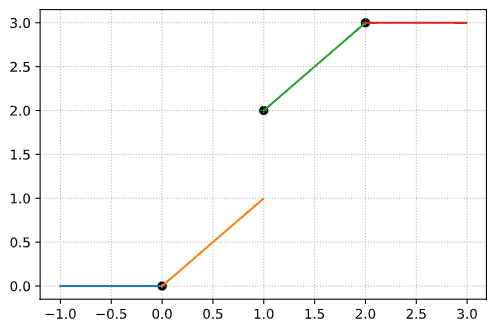
\includegraphics[width = 0.45 \textwidth]{3.1.1.png}
    }
    \hfill
    \subfloat[$G$]
    {
        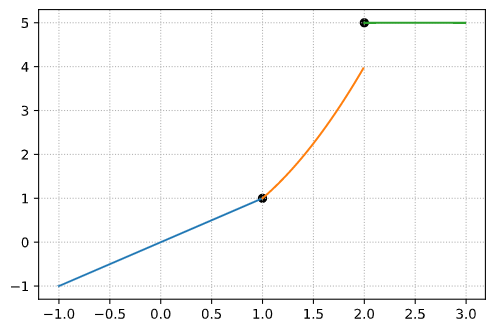
\includegraphics[width = 0.45 \textwidth]{3.1.2.png}
    }
    \caption{Verteilungsfunktionen $F$ und $G$ auf $[-1, 3]$}
    \label{fig:verteilungsfunktionen}
\end{figure}

\begin{align*}
    \begin{array}{c|c|c|c}
        x         & f   & G_\mathrm{c} & G_\mathrm{s} \\ \hline
        0 < x     & 0   & 0   & x   \\ \hline
        x = 0     & 0   & 0   & 0   \\ \hline
        0 < x < 1 & 1   & x   & 0   \\ \hline
        x = 1     & 0   & 1   & 0   \\ \hline
        1 < x < 2 & 2 x & x^2 & 0   \\ \hline
        x = 2     & 0   & 4   & 1   \\ \hline
        x > 2     & 0   & 4   & 1
    \end{array}
\end{align*}

\begin{enumerate}[label = \arabic*.]

    \item Bereich ($x < 0$):
    $F^\prime = 0$, $G^\prime = 0$

    \begin{align*}
        \implies & f = 0 \\
        \stackrel{\mathrm s_4}{\implies} & G_\mathrm{s}(x) = \int G^\prime(x) = x + ~\text{konst.}~ := x \\
        \implies & G_\mathrm{c}(x) = G(x) - G_\mathrm{s}(x) = x - x = 0
    \end{align*}

    \item Bereich ($x = 0$):
    $F$ springt, $G^\prime > 0$

    \begin{align*}
        \implies & f = 0 \\
        \stackrel{\mathrm c_1}{\implies} & G_\mathrm{c}(x) = G(x) - G(x - 0) + G_\mathrm{c}(x - 0) = x - x + 0 = 0 \\
        \implies & G_\mathrm{s}(x) = G(x) - G_\mathrm{c}(x) = 0 - 0 = 0
    \end{align*}

    \item Bereich ($0 < x < 1$):
    $F^\prime > 0$, $G^\prime > 0$

    \begin{align*}
        \implies & f = \frac{G^\prime(x)}{F^\prime} = \frac{1}{1} = 1 \\
        \stackrel{\mathrm c_3}{\implies} & G_\mathrm{c}(x) = \int G^\prime(x) = x + ~\text{konst.}, G_\mathrm{c}(0) = 0 \implies G_\mathrm{c}(x) = x \\
        \implies & G_\mathrm{s}(x) = G(x) - G_\mathrm{c}(x) = x - x = 0
    \end{align*}

    \item Bereich ($x = 1$):
    $F$ springt, $G$ springt

    \begin{align*}
        \implies & f = \frac{G(x) - G(x - 0)}{F(x) - F(x - 0)} = \frac{1^2 - 1}{\ast} = 0 \\
        \stackrel{\mathrm c_1}{\implies} & G_\mathrm{c}(x) = G(x) - G(x - 0) + G_\mathrm{c}(x - 0) = 1 - 1 + 1 = 1 \\
        \implies & G_\mathrm{s}(x) = G(x) - G_\mathrm{c}(x) = 1 - 1 = 0
    \end{align*}

    \item Bereich ($1 < x < 2$):
    $F^\prime > 0$, $G^\prime > 0$

    \begin{align*}
        \implies & f = \frac{G^\prime(x)}{F^\prime(x)} = \frac{2 x}{1} = 2 x \\
        \stackrel{\mathrm c_3}{\implies} & G_\mathrm{c}(x) = \int G^\prime(x) = x^2 + ~\text{konst.}, G_\mathrm{c}(1) = 1 \implies G_\mathrm{c}(x) = x^2 \\
        \implies & G_\mathrm{s}(x) = G(x) - G_\mathrm{c}(x) = x^2 - x^2 = 0
    \end{align*}

    \item Bereich ($x = 2$):
    $F^\prime = 0$, $G$ springt

    \begin{align*}
        \implies & f = 0 \\
        \stackrel{\mathrm s_2}{\implies} & G_\mathrm{s}(x) = G(x) - G(x - 0) + G_\mathrm{s}(x - 0) 5 - 2^2 + 0 = 1 \\
        \implies & G_\mathrm{c}(x) = G(x) - G_\mathrm{s}(x) = 5 - 1 = 4
    \end{align*}

    \item Bereich ($x > 2$):
    $F^\prime = 0$, $G^\prime = 0$

    \begin{align*}
        \implies & f = 0 \\
        \stackrel{\mathrm c_3}{\implies} & G_\mathrm{c}(x) = \int G^\prime(x) = ~\text{konst.}, G_\mathrm{c}(2) = 4 \implies G_\mathrm{c}(x) = 4 \\
        \implies & G_\mathrm{s}(x) = G(x) - G_\mathrm{c}(x) = 5 - 4 = 1
    \end{align*}

\end{enumerate}

\end{solution}

% -------------------------------------------------------------------------------- %
